\namedsection{ARM Cortex M0 Processor \label{sec:cortex}}{Pasat}

\note{talk about limitations of the processor ie no hardware divide or floating point arithmetic}

This section discusses one of the main requirement and one of the essential aspects of our project, ARM’s Cortex M0 processor. This processor is a member of the Cortex-M family and offers a great tradeoff in terms of costs and performance/functionality. It has been designed in order to allow intelligent compromises in terms of power usage, computational power and in the simplicity of the design. It implements a simplified version of the Advanced Microcontroller Bus Architecture (AMBA), the AMBA-Lite bus which allows connection to different peripherals. In this way, the Cortex-M0 generally acts as the master device and the peripherals act as slaves. In figure \ref{fig:cortexm0ds}, the schematic for the processor can be seen.\\
\begin{figure}
\centering
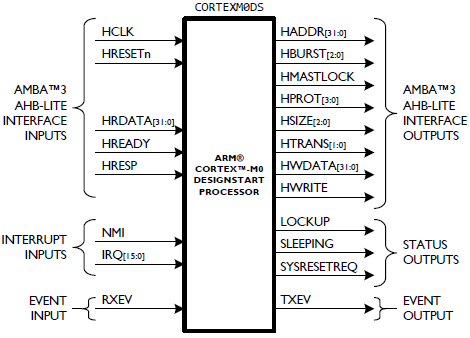
\includegraphics[scale=0.7]{figures/cortexm0ds_schematic.PNG}
\caption{Cortex M0DS schematic \label{fig:cortexm0ds}}
\end{figure}
\clearpage

\begin{figure}
\centering
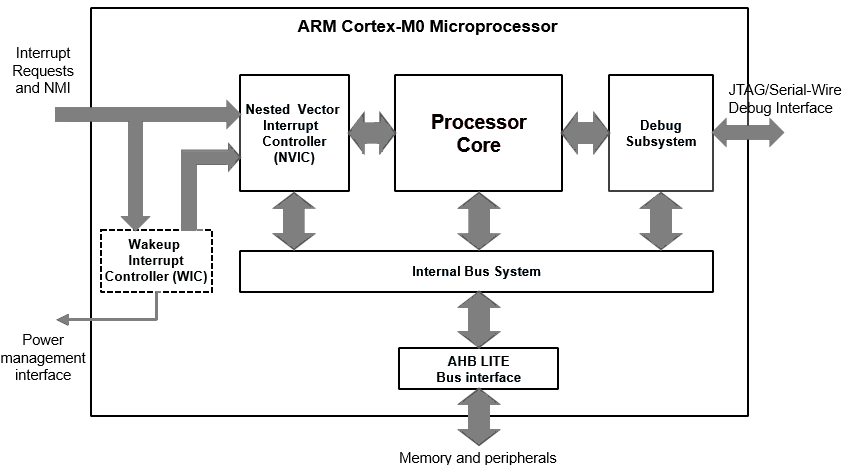
\includegraphics[scale=0.7]{figures/arm_cortexm0_microprocessor.PNG}
\caption{Cortex-M0 Block Diagram \label{fig:cortex_block}}
\end{figure}

The Cortex M0 has a 32-bit reduced instruction set computing(RISC) processor. It uses the ARMv6-M(Microcontroller), which is a subset of the ARMv7-M profile but it includes fewer instructions. The Cortex M0 is based on a Von-Neumann architecture, having both data and instructions share a single bus interface. It provides a Debug Extension that includes some architectural extensions to support debugging. The ARMv6-M offers support for 56 instructions as a subset of  Thumb-1(16-bit) and Thumb-2(16/32b-bit) which are present in the ARMv6T2. The Cortex M0 block diagram can be seen above in figure \ref{fig:cortex_block}. 

The Processor Core contains the internal registers, data path, ALU and control logics. The Cortex M0 has a three-stage pipeline: fetch, decode and exection and includes the 32-bit registers for general and special usages. The Cortex M0+ has only a two-stage pipeline to reduce the power usage.

The Nested Vectored Interrupt Controller(NVIC) handles up to 32 interrupts request signals and one NMI(Non-Maskable Interrupt). It also fulfils tasks such as comparing priorities between  interrupt requests and the current priority level. 

The Bus system contains the internal bus system, the data path in the processor core and the AHB LITE interface unit which is an on-chip bus protocol which enables some features required for high-performance, high clock frequency systems. 

The Debug system handles the program breakpoints, debugging control and the data watchpoints. This can put the processor in a  static state in order for the programmer to evaluate and analyse the status of the processor in that specific moment.

The Wakeup Interrupt Controller (WIC) is important for this project because it is used in low-power applications. The microcontroller can be set to enter sleep mode by turning off most of its components. If a interrupt request is sent, this component can inform the unit that handles the power management to power up the system.

Floating point is the formulaic representation for a real number for approximating it in order to obtain a balance between precision and range. Basically, it refers to the fact that a number's decimal point can "float", meaning  that is can be placed anywhere relative to significant digit from the number. One of the major challenges which were encountered in the use of the Cortex M0+ is the absence of floating point arithmetic on the device. This was mitigated by scaling each double value by $2^{12}$ and taking the integer part. After each multiplication, the value is bit-shifted by 12 to keep the scale factor consistent. This will be described late in more detail in section \ref{sec:floating-point}.

Real-time integer division supplied by ARM Libraries are faster then standard division routines for larger quotients, but slower for typical  quotients. Real time division is not available in the Cortex-M0+, so this was another issues that was overcome in our design. This was done by done by finding alternative methods to avoid division. More detail about this can also be found in \ref{sec:floating-point}.
\begin{figure}
\centering
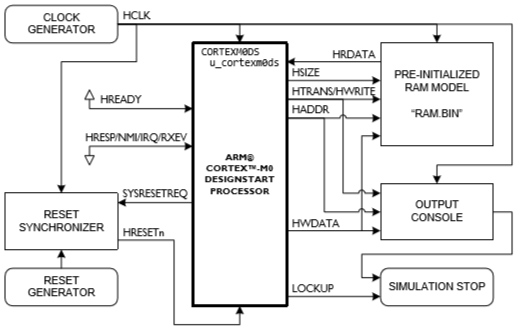
\includegraphics[scale=0.7]{figures/test_bench_schematic.PNG}
\caption{Cortex M0 test bench schematic} \label{fig:test_bench}
\end{figure}

Through ARM, we managed to gain access to a fixed configuration of the Cortex-M0 Processor known as Cortex-M0 DesignStart \cite{armdesignstart}. This simplified version offers us access to a Verilog version of the Cortex-M0 under the form of an obfuscated and preconfigured netlist, but it can be synthesized. This package offers us some Verilog codea test-bench which allow a simulation of the Cortex-M0 DesignStart module connected to a memory model and a clock and reset generator. It also include a basic C helloworld.c program. The schematic for the test-bench can be seen in figure \ref{fig:test_bench} and it connects the CORTEXM0DS to a memory model, a clock and a reset generators.

The tool used for simulating the test-bench is ModelSim, which is a tool that offers the possibility of simulating hardware description languages such as Verilog and VHDL. A new project must be created in ModelSim to which we add the Verilog files provided in the package, the test-bench and another binary file provided, ram.bin, which is an example memory image for the processor. The file is loaded at the beginning of the simulation by the test-bench.  The memory image is used for the helloworld.c program, which is used by the test-bench to write a message to the simulator's console and after that end the simulation. The result of the simulation can be seen in

Also, access was given to the CM0DS example design kit which contains various AHB-Lite peripherals and infrastructure components, useful to create complete systems. Before implementing the actual algorithm on the FPGA, a more basic simulation needs to be conducted on the platform to assure that it is compatible with the specific FPGA used. Next, the analysis of the sensors used for our project will be discussed. After that, discussions related to the about mBed platform which contains the Cortex M0+ and the Digilent Nexys4 FPGA board on which we aimed to implement the microprocessor as an extension will take place.
